%pygmentize_options: -O startinline=True

\chapter{Analysing PHP Code}

    The PHP programming language first appeared in 1995\cite{phphist}. Over the years 
    the language has evolved and so have the ways how programmers use it. 
    This project focuses on PHP version 5.5\footnote{From this point, 
    if the PHP version is not stated explicitly, it is implicitly 5.5.} 
    and the aim for the analysis 
    is to work well on PHP source code written in an object oriented style, 
    using modern PHP patterns and idioms that are described later in 
    this text. The analysis, however, should provide correct results for 
    any valid PHP code of any PHP version. We do not focus only on websites, but also on 
    PHP libraries and frameworks that by themselves do not contain 
    any PHP files that produce HTML or any other output for the user.
    
    \section{PHP semantics}
    This section describes some important parts of the semantics of 
    the PHP programming language, especially those that represent a 
    challenge for static analysis.
    
    \subparagraph*{}    
    In PHP, local or global variables, object fields and function or 
    method parameters are dynamically typed, which means that they 
    can hold values of completely different types at different 
    times of the execution.
    
    \subsection{Local Variables}
    Local variables in PHP do not need to be declared explicitly. 
    Instead the first usage of a variable is also its declaration. 
    If a variable's value is used before the variable got any 
    value assigned, then the interpreter generates a notice, 
    however the execution continues and value \code{null} is 
    used instead. A variable can get a value assigned to it when it 
    appears on a left hand side of an assignment or when a 
    reference to that variable is created, in which case it gets value 
    \code{null}, but no notice is generated. References are 
    discussed in one of the following subsections.

    The scope of a local variable is always its parent function not the 
    parent code block as in other languages like C or Java. 
    So in the following 
    example, the usage of variable \code{\$y} at the end 
    of the function can generate uninitialized variable notice, 
    however, if \code{\$x} was equal to \code{3}, 
    \code{\$y} will have a value although it 
    was declared in the nested code block.

%pygmentize_begin php
% function foo($x) {
%   if ($x == 3) { $y = 2; }
%   echo $y; // uninitialized variable if x != 3
% }
%pygmentize_end
\begin{Verbatim}[commandchars=\\\{\}]
 \PY{k}{function} \PY{n+nf}{foo}\PY{p}{(}\PY{n+nv}{\PYZdl{}x}\PY{p}{)} \PY{p}{\PYZob{}}
   \PY{k}{if} \PY{p}{(}\PY{n+nv}{\PYZdl{}x} \PY{o}{==} \PY{l+m+mi}{3}\PY{p}{)} \PY{p}{\PYZob{}} \PY{n+nv}{\PYZdl{}y} \PY{o}{=} \PY{l+m+mi}{2}\PY{p}{;} \PY{p}{\PYZcb{}}
   \PY{k}{echo} \PY{n+nv}{\PYZdl{}y}\PY{p}{;} \PY{c+c1}{// uninitialized variable if x != 3}
 \PY{p}{\PYZcb{}}
\end{Verbatim}
    
    \subsection{Global and Local Scope}
    PHP distinguishes two scopes for variables: global scope and 
    local scope. Local scope is a scope of local variables 
    within a user defined routine.         
    Variables that are declared 
    in global scope, that is outside of a user defined routine, 
    are available anywhere in global scope and are called 
    global variables. Global variables are also available 
    in user defined routines as long as they are imported 
    into the routine's scope using the keyword \code{global}.
    
%pygmentize_begin php
% $g1 = 1;  // global variables g1 and g2
% $g2 = 2;
% function foo() {
%   global $g1;
%   echo $g1;   // prints the value of global variable g1
%   $g2 = 4;   // sets the value of local variable g2,
%   // because global variable g2 was not imported, 
%   // its value does not change
% }
%pygmentize_end
\begin{Verbatim}[commandchars=\\\{\}]
 \PY{n+nv}{\PYZdl{}g1} \PY{o}{=} \PY{l+m+mi}{1}\PY{p}{;}  \PY{c+c1}{// global variables g1 and g2}
 \PY{n+nv}{\PYZdl{}g2} \PY{o}{=} \PY{l+m+mi}{2}\PY{p}{;}
 \PY{k}{function} \PY{n+nf}{foo}\PY{p}{()} \PY{p}{\PYZob{}}
   \PY{k}{global} \PY{n+nv}{\PYZdl{}g1}\PY{p}{;}
   \PY{k}{echo} \PY{n+nv}{\PYZdl{}g1}\PY{p}{;}   \PY{c+c1}{// prints the value of global variable g1}
   \PY{n+nv}{\PYZdl{}g2} \PY{o}{=} \PY{l+m+mi}{4}\PY{p}{;}   \PY{c+c1}{// sets the value of local variable g2,}
   \PY{c+c1}{// because global variable g2 was not imported, }
   \PY{c+c1}{// its value does not change}
 \PY{p}{\PYZcb{}}
\end{Verbatim}

    Global variables can be imported and used in any user defined 
    routine. This means that even if we know some type information 
    about a global variable's value at some point in the analysed 
    code (e.g. straight after assignment to that variable), 
    any time another user defined routine is invoked, we 
    have to take into account that the other routine can 
    change the value of the global variable even if we do not 
    pass the global variable to the invoked routine 
    as an argument passed by reference.

    \subsection{Closures}
    PHP also supports anonymous functions. An anonymous function has its 
    own scope as any other function and its local variables are not visible 
    to the scope where it was declared. Variables from the parent 
    scope are available in the closure scope only if they are 
    explicitly imported to its scope and they can be captured 
    by value or by reference. Only the later represents a 
    challenge for the analysis, because any code that can 
    access the closure can invoke it and thus change the 
    values of variables imported to the closure's scope 
    by reference. By invoking a closure, we can influence 
    the values of variables in a completely different 
    and otherwise inaccessible scope.
    
    \subsection{References}
    References in PHP are similar, but not same, as pointers 
    in the C programming language. PHP has a special 
    operator \code{=\&} (assign by reference) that turns 
    the variable on the 
    left hand side into a reference to the 
    variable on right hand side. For example \code{\$a=\&\$b}, 
    after this, any assignment 
    to \code{\$a} will in fact change the 
    value of \code{\$b} and wherever 
    the value of \code{\$a} is used (e.g. in an expression), 
    the value of \code{\$b} is used instead.
    
    The variable where the reference is pointing to is determined 
    in a transitive fashion, which means that if we assign 
    by reference another reference, the new reference will 
    point to where the other reference was pointing to, 
    but the intermediate link is lost. The following example 
    illustrates this.
    
%pygmentize_begin php
% $a =& $b;       // a points to b
% $c =& $a;       // c points to where a points, that is b
% $a =& $d;       // a points to d, but c still points to b
%pygmentize_end    
\begin{Verbatim}[commandchars=\\\{\}]
 \PY{n+nv}{\PYZdl{}a} \PY{o}{=\PYZam{}} \PY{n+nv}{\PYZdl{}b}\PY{p}{;}       \PY{c+c1}{// a points to b}
 \PY{n+nv}{\PYZdl{}c} \PY{o}{=\PYZam{}} \PY{n+nv}{\PYZdl{}a}\PY{p}{;}       \PY{c+c1}{// c points to where a points, that is b}
 \PY{n+nv}{\PYZdl{}a} \PY{o}{=\PYZam{}} \PY{n+nv}{\PYZdl{}d}\PY{p}{;}       \PY{c+c1}{// a points to d, but c still points to b}
\end{Verbatim}

    \subsection{Arrays}
    Arrays in PHP do not have to be homogenous and 
    they can be indexed by either integers or strings.
    In fact, PHP arrays are hash maps rather than arrays 
    in the usual sense and that is also how they are 
    implemented internally. 
    
    String indexed heterogenous arrays are often used 
    as flexible ad-hoc structured data type. 
    Instead of defining a class 
    with required fields, one can use what would be a 
    field name as an index into an array. Such arrays 
    are usually indexed only with finite number of 
    constant string values. 
    
    In this light, it is no 
    surprise that using the subscribe operator 
    \code{[]} with string index on an object instance will 
    access the field with the same name as the index value.

    \subsection{Interesting Control Flow Structures}
    The \code{break} and \code{continue} statements with 
    optional numeric argument are supported in PHP in a 
    similar way as in other standard imperative programming 
    languages. There are, however, important differences 
    to be noted.
    
    Firstly, The numeric argument can be an arbitrary 
    expression in some of the older versions of PHP, in which 
    case we cannot statically determine the target of 
    the jump for the control flow resolution.
    
    Secondly, the \code{switch} statement is considered 
    a loop for the purposes of both \code{break} and 
    \code{continue}. The semantics of \code{break} 
    is intuitive. One of the meaningful use cases is to 
    break a loop from within a \code{switch} by 
    using \code{break 2}. The semantics of 
    \code{continue} statement 
    is perhaps not so intuitive: within a \code{switch} 
    it works the same way as \code{break}.
    
    \subparagraph*{Switch Statement Semantics.} 
    The basic semantics of the \code{switch} statement in PHP is 
    again very similar to that of other standard imperative 
    programming languages. The \code{switch} statement in PHP 
    permits an arbitrary expression as the value to be used 
    for comparison with values of its \code{case} labels. Furthermore, 
    the values of \code{case} labels can also be arbitrary 
    expressions and because we are in a context of dynamic 
    programming language, they can again evaluate to a value 
    of any type.
    
    At runtime, the switch expression is evaluated only once 
    at the beginning, and if it has an undefined value (undefined variable, 
    void function call), then the control flow goes directly 
    to the default item, without evaluating the expressions 
    in the case items. If the value is defined, then it is 
    one by one compared to the values that the 
    \code{case} labels evaluate to. If a \code{case} label evaluates 
    to \code{boolean} value, then it is used to decide whether to 
    jump to that \code{case} item or continue with evaluating 
    the value of the next \code{case} label. Note that the value of 
    switch expression is not compared to the \code{case} label value. 
    If a \code{case} label evaluates to a complex type (\code{object} or \code{array}), 
    it is ignored and evaluation continues with the next \code{case} label. 
    And finally, if a \code{case} label evaluates to an 
    \code{integer}, \code{float} or \code{string} value, it is 
    compared to the switch expression. All these expressions can 
    have side effects due to usage of assignments as expressions 
    or calls of functions with side effects. 
    
    PHP also allows to place the \code{default} label anywhere in between 
    the other \code{case} labels. This can be used for fall-back 
    to or from a \code{case} item as in the following code sample 
    that is abbreviated version of actual code taken from the 
    WordPress\cite{wordpress} code base.
    
%pygmentize_begin php
%switch ( $status ) {
%    default:
%    case 'install':
%        $actions[] = '<a class="install-now" ...';
%        break;
%    case 'update_available':
%        $actions[] = '<a class="install-now" ...';
%        break;
%    case 'newer_installed':
%    case 'latest_installed':
%        $actions[] = '<span class="install-now" ...';
%        break;
%}
%pygmentize_end    
\begin{Verbatim}[commandchars=\\\{\}]
\PY{k}{switch} \PY{p}{(} \PY{n+nv}{\PYZdl{}status} \PY{p}{)} \PY{p}{\PYZob{}}
    \PY{k}{default}\PY{o}{:}
    \PY{k}{case} \PY{l+s+s1}{\PYZsq{}install\PYZsq{}}\PY{o}{:}
        \PY{n+nv}{\PYZdl{}actions}\PY{p}{[]} \PY{o}{=} \PY{l+s+s1}{\PYZsq{}\PYZlt{}a class=\PYZdq{}install\PYZhy{}now\PYZdq{} ...\PYZsq{}}\PY{p}{;}
        \PY{k}{break}\PY{p}{;}
    \PY{k}{case} \PY{l+s+s1}{\PYZsq{}update\PYZus{}available\PYZsq{}}\PY{o}{:}
        \PY{n+nv}{\PYZdl{}actions}\PY{p}{[]} \PY{o}{=} \PY{l+s+s1}{\PYZsq{}\PYZlt{}a class=\PYZdq{}install\PYZhy{}now\PYZdq{} ...\PYZsq{}}\PY{p}{;}
        \PY{k}{break}\PY{p}{;}
    \PY{k}{case} \PY{l+s+s1}{\PYZsq{}newer\PYZus{}installed\PYZsq{}}\PY{o}{:}
    \PY{k}{case} \PY{l+s+s1}{\PYZsq{}latest\PYZus{}installed\PYZsq{}}\PY{o}{:}
        \PY{n+nv}{\PYZdl{}actions}\PY{p}{[]} \PY{o}{=} \PY{l+s+s1}{\PYZsq{}\PYZlt{}span class=\PYZdq{}install\PYZhy{}now\PYZdq{} ...\PYZsq{}}\PY{p}{;}
        \PY{k}{break}\PY{p}{;}
\PY{p}{\PYZcb{}}
\end{Verbatim}
    
    
    \subsection{Conditional Declarations}
    User defined functions, classes, etc. are declared in 
    a global scope in PHP, that is a scope where one can 
    as well place any arbitrary code. Therefore a declaration 
    can be wrapped in any control structure. 
    It is not allowed to redeclare once declared symbol, however.
    
    A typical use case is to dynamically import a file 
    that may provide some functions and then check, 
    using \code{function\_exists}, whether the functions were 
    indeed declared and if not, provide default implementation.
    This is a pre-object-oriented way of doing overriding and 
    is usually not to be found in modern projects. Nonetheless, 
    WordPress still relies on this pattern in parts of its code base.
    
    Although the mentioned pattern could be deemed as 
    reasonable and useful. This feature allows 
    to write very problematic code as in the following example 
    that may or may not crash on fatal errors ``Cannot 
    redeclare foo()'' or ``Call to undefined function foo()'' 
    depending upon the user input.
    
%pygmentize_begin php
%while ($_POST['a'] != 3) {
%   function foo() { return 5; }
%   $_POST['a'] = $_POST['b'];
%}
%echo foo();
%pygmentize_end        
\begin{Verbatim}[commandchars=\\\{\}]
\PY{k}{while} \PY{p}{(}\PY{n+nv}{\PYZdl{}\PYZus{}POST}\PY{p}{[}\PY{l+s+s1}{\PYZsq{}a\PYZsq{}}\PY{p}{]} \PY{o}{!=} \PY{l+m+mi}{3}\PY{p}{)} \PY{p}{\PYZob{}}
   \PY{k}{function} \PY{n+nf}{foo}\PY{p}{()} \PY{p}{\PYZob{}} \PY{k}{return} \PY{l+m+mi}{5}\PY{p}{;} \PY{p}{\PYZcb{}}
   \PY{n+nv}{\PYZdl{}\PYZus{}POST}\PY{p}{[}\PY{l+s+s1}{\PYZsq{}a\PYZsq{}}\PY{p}{]} \PY{o}{=} \PY{n+nv}{\PYZdl{}\PYZus{}POST}\PY{p}{[}\PY{l+s+s1}{\PYZsq{}b\PYZsq{}}\PY{p}{];}
\PY{p}{\PYZcb{}}
\PY{k}{echo} \PY{n+nx}{foo}\PY{p}{();}
\end{Verbatim}
    
                
    \subsection{Auto-loading}
    Historically, in PHP in order to reference any symbol 
    from a different file, one had to import that 
    file explicitly. Newer versions of PHP support  
    customized auto-loading. A used defined routine 
    can be invoked by the runtime every time an 
    undefined class is referenced. 
    The auto-loading routine is then responsible for 
    importing the file(s) that contain the code of the 
    required class. 
    
    Auto-loading routine can use arbitrary logic to 
    determine what file(s) to import, in fact, it can 
    execute arbitrary code. Typical 
    pattern used for example in 
    Zend Framework\cite{zendframework} before namespaces were 
    introduced to PHP is to have a file per class and use 
    class names in form of 
    \code{CodeFolder1\_SubFolderName\_FileName} for 
    a class placed in file 
    \filepath{CodeFolder1\SubFolderName\FileName.php}.
    
    \subsection{PHPDoc Annotations}
    Although not part of the official PHP syntax, 
    there is a widely recognized format for documentation 
    comments of JavaDoc style called PHPDoc. PHPDoc comments 
    may contain type information that cannot be expressed using 
    PHP syntax. For example, PHP allows ``type hints'' 
    for routine parameters, but only for class types, 
    not for primitive types like \code{int}. However, 
    primitive type expectations can be included in the 
    documentation comments. The important difference 
    is that PHP will throw an exception at runtime if 
    a routine is invoked with a parameter of different 
    type than what its ``type hint'' is. The documentation
    comments, on the other hand, are of course ignored 
    by the runtime.
    
    The PHPDoc defines a fairly advanced syntax for expressing 
    type information. It supports multiple 
    primitive and class types, homogenous and heterogenous arrays as well 
    multidimensional arrays, and some constants like \code{false}.
    For example, in the following code the documentation 
    comment tells us that function \code{foo} can return 
    either \code{null}, or \code{false} (but should never 
    return \code{true}), or an array of \code{integer} values.
    
%pygmentize_begin php
% /**
%  * @return null|false|int[]
%  */
% function foo() { ...
%pygmentize_end
\begin{Verbatim}[commandchars=\\\{\}]
 \PY{l+s+sd}{/**}
\PY{l+s+sd}{  * @return null|false|int[]}
\PY{l+s+sd}{  */}
 \PY{k}{function} \PY{n+nf}{foo}\PY{p}{()} \PY{p}{\PYZob{}} \PY{o}{...}
\end{Verbatim}
    
    \section{Static Code Analysis}       
        Static analysis of source code is an analysis that is performed without 
        executing the code. This means that we do not need to have a
        web server, for example, in order to analyse code of a web application. 
        We can also guarantee some properties of the analysis that would not 
        be possible to guarantee if we executed the code. Namely the halting property and 
        upper bounds on time and space complexity. Arbitrary code may not 
        halt if executed, but static analysis of such code can still halt 
        and give results.
        
        Static analysis can be used to get possible types of an expression in 
        a dynamically typed language, to find out expressions that have constant 
        value through constant propagation and many other problems. 
        Static analyses usually do not give accurate solution, but 
        its approximation, which can be an over-approximation or 
        an under-approximation and it is up to the designer and user of the analysis 
        which one is acceptable for his or her\footnote{``His'' or ``he'' 
        should be read as ``his or her'' or ``he or she'' through the rest of the text.} 
        purposes.

        Data Flow Analysis (DFA)\cite{aho1985compilers}, \cite{nielson1999principles} has 
        become a de-facto standard type of analysis for most of the optimizing compilers and 
        other more complex static analyses are either directly based on DFA or on 
        the ideas behind DFA. DFA is also used in Control Flow for Phalanger. 
        In the rest of this section, we provide brief description of 
        firstly DFA in general and then how we have leveraged DFA for 
        the purposes of PHP code analysis.
        
        %---------------------------------------------------------------------------------------
        \subsection{Program State}
        Execution of a program can be seen as a series of transformations of 
        the program state. Each individual program instruction, when executed, 
        can change the program state and produces its \emph{output state}.         
        How exactly is defined by the instruction's semantics and it typically 
        depends on the \emph{input state}, which is a program state produced 
        by the previously executed instruction. 
        
        The goal of a static analysis is to devise some useful piece of information 
        about how instruction $i$ can change the program state, so that it can 
        be used for program optimization or to reveal potentially problematic 
        instructions. For example, if assignment $a=4/b$ always assigns 
        constant value $1$ to $a$, because $b$ happens to be equal to $4$ 
        in any possible program state preceding $a=4/b$, we can change 
        $a=4/b$ to $a=1$, which has the same affect to the program state. 
        If we instead found out that $b$ is always equal to $0$, we would 
        know that this instruction will cause an exception.
        
        The result we expect from a static analysis is, for each instruction 
        in the program, provide some useful property of program state transformation 
        that always holds every time the instruction is executed. 
        The analyses differ in the properties they compute. 
        We will call such computed property a \emph{data-flow}.
        
        
        %---------------------------------------------------------------------------------------
        \subsection{Control Flow Graph.} 
        DFA is typically performed on a control flow graph, 
        although there exist approaches to DFA 
        without explicit control flow graph 
        construction \cite{mohnen2002graph}.
        
        Control flow graph nodes, also called basic blocks, 
        are program statements that are always executed sequentially. 
        Directed edges represent the control flow between basic blocks, 
        for example, jumps in the control flow due to conditionals, 
        \code{goto} statements or any other statements that can change 
        the flow of the program.        
        Control flow graphs usually contain two special nodes: 
        entry node and exit node. The entry node does not have any 
        incoming edges and all the paths lead to the exit node.        
        An example of a control flow graph is given in figure \ref{cfg}.
        
\begin{table}[h]
  \begin{tabular}{ l | m{6cm} }
  \centering
    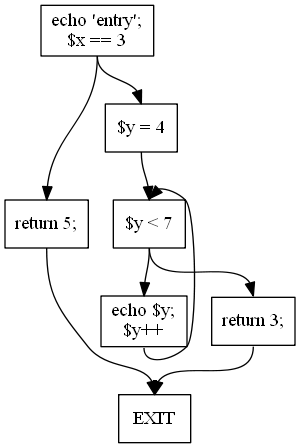
\includegraphics[scale=0.7]{img/cfg.png}
  &
 
\begin{minipage}{6cm}
%pygmentize_begin php
%   echo 'entry';
%   if ($x == 3)
%       $y = 4;
%   else
%       return 5;
%        
%   while ($y < 7) {
%       echo $y;
%       $y++;
%   }
%
%   return 3;
%pygmentize_end
\begin{Verbatim}[commandchars=\\\{\}]
   \PY{k}{echo} \PY{l+s+s1}{\PYZsq{}entry\PYZsq{}}\PY{p}{;}
   \PY{k}{if} \PY{p}{(}\PY{n+nv}{\PYZdl{}x} \PY{o}{==} \PY{l+m+mi}{3}\PY{p}{)}
       \PY{n+nv}{\PYZdl{}y} \PY{o}{=} \PY{l+m+mi}{4}\PY{p}{;}
   \PY{k}{else}
       \PY{k}{return} \PY{l+m+mi}{5}\PY{p}{;}
        
   \PY{k}{while} \PY{p}{(}\PY{n+nv}{\PYZdl{}y} \PY{o}{\PYZlt{}} \PY{l+m+mi}{7}\PY{p}{)} \PY{p}{\PYZob{}}
       \PY{k}{echo} \PY{n+nv}{\PYZdl{}y}\PY{p}{;}
       \PY{n+nv}{\PYZdl{}y}\PY{o}{++}\PY{p}{;}
   \PY{p}{\PYZcb{}}

   \PY{k}{return} \PY{l+m+mi}{3}\PY{p}{;}
\end{Verbatim}
\end{minipage}

  \\
  \end{tabular}
  \caption{Control flow graph\label{cfg}}  
\end{table}        
        
        %---------------------------------------------------------------------------------------
        \subsection{Transfer functions}
        
        We say that the input state of a statement is associated with 
        the \emph{program point before} the statement and the output state 
        is associated with the \emph{program point after} the statement. 
        Our aim is to calculate \emph{data-flow} value for both 
        program points for each statement, denoted $IN(s)$ and $OUT(s)$ for 
        a statement $s$.
        
        \subsubsection*{Single Statement}
        
        We can express the \emph{data-flow} for \emph{program point after} 
        a statement as a function of the \emph{data-flow} of 
        \emph{program point before} the statement, also called \emph{transfer function}. 
        Formally if $f_t$ is a \emph{transfer function}, then $f_t(IN(s))=OUT(s)$.
        Each type of statement will have a different \emph{transfer function} 
        that will reflect the semantics of the statement. 
        
        \emph{Transfer functions} are often described in the form of inference rules. 
        An example of an inference rule can be 
        ``if the type of variable \code{b} is \code{Integer} in state $S_1$, 
        then after executing statement \code{a=b}, we get a new state $S_2$ that 
        is the same as $S_2$ except variable \code{a} is of type \code{Integer} in $S_2$''. 
        Those rules can be more formally described with the following notation        
        $$
        \infer{[a=b, S_1] \rightarrow S_2, S_2 \vdash a : Integer}{S_1 \vdash b : Integer}
        $$        
        where above the horizontal line we have hypothesis and below is 
        the conclusion. The exact notation is not important, we will be using it 
        intuitively to illustrate the ideas that we describe.
        
        \subsubsection*{Statements Interaction}
        
        The \emph{data-flow} for \emph{program point before} a statement 
        depends on the \emph{data-flow} of \emph{program point after} the 
        last executed statement. Let us consider a basic block $B$ with 
        statements $s_0, s_1, ..., s_n$.
        
        In the case of any $s_i \neq s_0$, that is any statement but 
        the first one, there is only one statement whose execution 
        can precede the execution of $s_i$ and that is the previous statement 
        in the sequence: $s_{i-1}$. So we have $IN(s_i) = OUT(s_{i-1})$ 
        for $i\in{[1..n]}$. 
        
        In fact, thanks to this property, we can define \emph{transfer function} 
        $f_B$ of a basic block as composition of transfer functions of 
        its statements. Formally: 
        
        \[ f_B = f_{s_n} \circ f_{s_{(n-1)}} \circ ... f_{s_0} \]
        
        where $f_{s_i}$ is the transfer function for statement $s_i$.            
        Furthermore, we denote \emph{data-flow values} of basic block as 
        $IN(B)=IN(s_1)$ and $OUT(B)=OUT(s_n)$. From the definitions we can 
        observe simple identities: 
        
        \[ f_B(IN(s_1))=f_B(IN(B))=OUT(B)=OUT(s_n) \]
        
        The first statement $s_1$ of the basic block has to be 
        handled differently. Its execution can be preceded by 
        execution of the last statement of any of 
        the basic blocks $B_1, B_2, ..., B_m$ that precede basic block 
        $B$ in the control flow graph. One of the possibilities to deal with 
        this, is to combine \emph{data-flows} $OUT(B_1), ..., OUT(B_m)$ into 
        single \emph{data-flow} that approximates all of them. 
        Nonetheless, the way the \emph{data-flows} are combined depends 
        on the concrete \emph{data-flow} type and thus 
        should be defined by the analysis. We denote the function to 
        combine \emph{data-flows} as $\mathit{MEET}$. 
        
        \subsubsection*{Equations for Data-Flow}
        
        If we put everything together, we get a set of equations:
        \begin{align*}
            OUT(B_i) &= f_{B_i}(IN(B_i)) \\
            IN(B_i) &= \mathit{MEET}(OUT(P_0), ..., OUT(P_m)) \\ 
        \end{align*}
        where $P_i$ is predecessor of $B_i$ in the control flow graph. 
        The analysis must also define value of $IN(START)$, that is 
        \emph{input state} for the initial node, which does not have 
        any predecessors.
        
        \subsubsection*{Example}
        We will illustrate the system of \emph{data-flow} equations on a 
        simple example. The subject of our analysis will be the 
        type of the variable \code{\$i} in the code sample in figure \ref{dfacfg}.
        
        \emph{Data-flow} will be a set of possible types of variable $i$ and 
        initial \emph{data-flow} of the start node will be an empty set.

\begin{table}[h]
  \begin{tabular}{ l | m{6cm} }
  \centering
    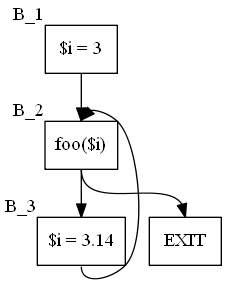
\includegraphics[scale=0.7]{img/dfa-cfg.png}
  &
 
\begin{minipage}{6cm}
%pygmentize_begin php
%   $i = 3;
%   while (foo($i)) {
%       $i = 3.14;
%   }
%   // exit
%pygmentize_end
\begin{Verbatim}[commandchars=\\\{\}]
   \PY{n+nv}{\PYZdl{}i} \PY{o}{=} \PY{l+m+mi}{3}\PY{p}{;}
   \PY{k}{while} \PY{p}{(}\PY{n+nx}{foo}\PY{p}{(}\PY{n+nv}{\PYZdl{}i}\PY{p}{))} \PY{p}{\PYZob{}}
       \PY{n+nv}{\PYZdl{}i} \PY{o}{=} \PY{l+m+mf}{3.14}\PY{p}{;}
   \PY{p}{\PYZcb{}}
   \PY{c+c1}{// exit}
\end{Verbatim}
\end{minipage}

  \\
  \end{tabular}
  \caption{Code for Data-Flow Example\label{dfacfg}}  
\end{table}

        \emph{Transfer functions}: we will assume that function call does 
        not change state, therefore the transfer function of 
        function call is identity -- $OUT(s)=IN(s)$. Assignment of 
        a constant \code{c} of type \code{T} to \code{\$i} changes 
        type of \code{\$i} to \code{T}.
        
        \emph{MEET} operation will be union of the sets of 
        possible types of \code{\$i}.
        
        The set of equations is in this case
        
        \begin{align*}
            OUT(B_1) &= f_{B_1}(IN(B_1))=f_B(\emptyset) \,\,\,\,\,\text{(initial node)} \\
            OUT(B_2) &= f_{B_2}(\mathit{MEET}(OUT(B_1), OUT(B_3))) \\
            OUT(B_3) &= f_{B_3}(OUT(B_2))     
        \end{align*}
        
        Knowing that $f_{B_1}$ and $f_{B_3}$ are constant functions, because 
        the assignment changes type of \code{\$i} to \code{T} without taking 
        the \emph{input data-flow} into account, and $f_{B_2}$ is identity 
        function, we can simplify the equations to

        \begin{align*}
            OUT(B_1) &= \left\{ \mathit{Integer} \right\} \\
            OUT(B_2) &= f_{B_2}(\mathit{MEET}(OUT(B_1), OUT(B_3))) \\
            OUT(B_3) &= \left\{ \mathit{Double} \right\} \\
            \\
            OUT(B_1) &= \left\{ \mathit{Integer} \right\} \\
            OUT(B_2) &= f_{B_2}( \left\{ \mathit{Integer} \right\} \cup \left\{ \mathit{Double} \right\} ) = 
                \left\{ \mathit{Integer}, \mathit{Double} \right\} \\
            OUT(B_3) &= \left\{ \mathit{Double} \right\}
        \end{align*}
        
        With this result we can, for example, check that function \code{foo} 
        is invoked with correct argument type, because from $IN(B_2)$ we 
        know that \code{\$i} at the moment of invocation of \code{foo} 
        can be either of type \code{Integer} or \code{Double}.
                
        \subsection{Finding Solution for the Data-flow Equations}
        
        \subsubsection*{Lattices.}
        The algorithm for finding a solution to a set of data-flow 
        equations is based on algebraic structures called lattices. 
        A lattice is a partially ordered set in which every 
        two elements have a least upper bound, called supremum, 
        and a greatest lower bound, called infimum.
        
        \emph{Bounded lattice} is a lattice that has 
        a greatest element and a least element, 
        usually denoted as $\top$ and $\bot$. 
        A bounded lattice is depicted in figure \ref{lattice}.       
        
\begin{figure}[h]  
  \centering
    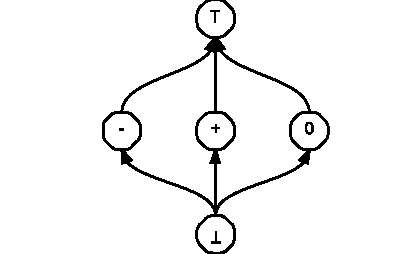
\includegraphics{img/lattice.pdf}
  \caption{Bounded lattice with 5 elements.\label{lattice}}    
\end{figure}

        There are several properties of lattices important for DFA.
        
        If we have a finite bounded lattice $(S, \leq_{s})$ and a function 
        $f:S\rightarrow{S}$ that is monotonous, in order words, 
        $\forall{a,b\in{S}}: a\leq_s{b} \Rightarrow f(a)\leq_s{f(b)}$, 
        then $\forall{x\in{S}}$ $\exists{k\in\mathbb{N}}$, such that 
        $f^k(x)=f^{(k+1)}(x)$. $f^k(x)$ is called a fixpoint.
        
        Intuitively, $f$ has to have a fixpoint because 
        for every argument $y$, it must either return 
        $y$ itself, but then $y$ is a fixpoint, or it 
        returns another element that is strictly 
        greater than $y$, but this cannot go on forever, because eventually 
        $f$ will be given $\top$ for which it does not have 
        any other option but returning $\top$ and we 
        have a fixpoint again.
        
        From this property further follows that if we use finite 
        lattice's elements as a domain for transfer functions, 
        and the transfer functions are monotonous, then the set of 
        data-flow equations has a solution, which is a safe 
        approximation of the, in a sense, best solution to the 
        data flow problem. Details can be found in \cite{kildall1973unified}.
        
        Product lattice obtained from two or more lattices 
        is also a lattice, which can simplify the design of 
        data flow analyses.

        Power set $\mathcal{P}(S)$, the set of all subsets of $S$, 
        is also a lattice, the lattice order relation 
        being subset relation $\subseteq$.

        \subsubsection*{The Iterative Algorithm}
        
        The algorithm to find the solution to the data-flow equations 
        initially sets $OUT(B_i)$ for every basic block to the initial 
        \emph{data-flow}, which should be the lowest element of the lattice. 
        Then it iteratively takes a basic block $B_j$ such that 
        its input \emph{data-flow} $IN(B_j)$ has changed or is not 
        initialized yet and computes $OUT(B_j)$, which might change 
        the input \emph{data-flow} of the ancestors of $B_j$. 
        The process is repeated until a the system stabilizes. 
        
        The algorithm can take basic blocks in any order, however, 
        the reverse post order provides the best time complexity 
        \cite{aho1985compilers}.
        
        \subsubsection*{Bit Vectors as Data-flow Representation}

        The performance of the algorithm also depends on the implementation 
        of \emph{data-flow}, the $\textit{MEET}$ operations and the transfer 
        functions. 
        
        \emph{Data-flow} often represents a subset of a set of possible values 
        and the $\textit{MEET}$ operation is either union or intersection.
        For example, subset of all possible types of a variable. 
        Furthermore, we want to calculate the information for all 
        variables not only for one. If we know the number of variables $n$ and 
        types $m$ in advance, we can represent the \emph{data-flow} as 
        a bit-vector where groups of $m$ bits represent a data of 
        single variable and within those bits, value of bit with 
        index $i$ indicates whether the type with index $i$ is in the set. 
        Union or intersection can be implemented using fast bitwise operations.


        % -----------------------------------------------------------------------
        \subsection{Abstraction}
        
        The \emph{data-flow} value for program point is typically an abstraction 
        of some property of the set of all possible program states that can be 
        observed during real execution for that program point. 
        
        Abstracting the desired property is often important in order to make 
        the analysis practical or even feasible. Let us consider an analysis 
        that should determine a sign of integral variables at each program point.
        We can have inference rules of the following form.
        
        $$
        \infer{[v_3=v_1+v_2, S_1] \rightarrow S_2, S_2 \vdash v_3 : -7 (sign: \ominus)}
        {S_1 \vdash v_1 : -10 (sign: \ominus) & S_1 \vdash v_2 : 3 (sign: \oplus)}
        $$
        
        However, the implementation would not be very efficient and also the full 
        information about variables values is not always available, but in some cases 
        we can deduce another less precise, but still useful piece of information 
        by other means. For example, variable of type \code{unsigned integer} will 
        always be positive, we can count on that even if we do not know the actual value. 
        What we can do is to abstract the possible integral values with set 
        $\{0, \ominus, \oplus\}$ with the following meanings         
        \begin{itemize}
            \item $\ominus$ represents all negative integers,
            \item $\oplus$ represents all positive integers,
            \item $0$ represents zero,
        \end{itemize}                
        and rewrite the inference rules as follows:
        
        $$
        \infer{[v_3=v_1+v_2, S_1] \rightarrow S_2, S_2 \vdash v_3 : \ominus}
        {S_1 \vdash v_1 : \ominus & S_1 \vdash v_2 : \ominus}
        $$
        
        Nonetheless, there is another problem. What to do when we have $\ominus$ 
        and $\oplus$ in the hypothesis.
        
        $$
        \infer{[v_3=v_1+v_2, S_1] \rightarrow S_2, S_2 \vdash v_3 : ?}
        {S_1 \vdash v_1 : \ominus & S_1 \vdash v_2 : \oplus}
        $$
        
        The solution is to extend the domain so that it is closed under all operations. 
        We add another element to our set:
        \begin{itemize}
            \item $\top$ represents an unknown value (either positive, negative, or zero).
        \end{itemize}
        Then the rule will be:
        
        $$
        \infer{[v_3=v_1+v_2, S_1] \rightarrow S_2, S_2 \vdash v_3 : \top}
        {S_1 \vdash v_1 : \ominus & S_1 \vdash v_2 : \oplus}
        $$        
        
        And for example another rule dealing with $\top$ in hypothesis:
        $$
        \infer{[v_3=v_1+v_2, S_1] \rightarrow S_2, S_2 \vdash v_3 : \top}
        {S_1 \vdash v_1 : \ominus & S_1 \vdash v_2 : \top}
        $$
        
        It is no surprise that we used symbol $\top$, which is also used to denote the 
        greatest element in a lattice. By adding $\bot$, the least element, and inference 
        rules for it, we can get a lattice depicted in \ref{lattice} and use 
        this abstraction as \emph{data-flow} value.
        
        \subsubsection*{Formalization}

        There is a theoretical framework for designing sound and correct 
        abstractions. In a nutshell, an abstraction following this framework 
        has to include: 
        
        \begin{itemize*}
            \item concrete domain $C$, which has to be a lattice ,
            \item abstract domain $A$, which has to be a finite lattice,
            \item concretization function $\gamma{}:A\mapsto{}C$,
            \item abstraction function $\alpha{}:C\mapsto{}A$,
        \end{itemize*}
        
        In our case the concrete domain could be the power set of all 
        possible integral values, which is a lattice, and the abstract 
        domain with elements $\{0, \ominus, \oplus\, \top, \bot\}$ was 
        described above. The $\gamma$ and $\alpha$ functions map values 
        from one domain to another. When we map elements of concrete domain 
        to the abstract domain, we loose precision due to abstraction. 
        Let us provide few examples, instead of a formal definition 
        of $\gamma$ and $\alpha$.
        
        \begin{align*}
            \begin{split}
                \gamma{}(\oplus) &= \left\{1, 2, 3, ...\right\} \\
                \gamma{}(\top) &= \top = \left\{..., -2, 1, 0, 1, 2, ...\right\} \\
            \end{split}
            \begin{split}
                \alpha{}(\left\{3, 4, 5\right\}) &= \oplus \\ 
                \alpha{}(\left\{3, -4\right\}) &= \top \\
            \end{split}
        \end{align*}
        
        The framework for abstract interpretation further defines 
        necessary conditions for the $\gamma$ and $\alpha$ functions 
        and conditions for the \emph{transfer functions} with respect 
        to $\gamma$ and $\alpha$ mapping. Details and other 
        static analysis methods based on abstract interpretation 
        framework can be found in \cite{cousot1977abstract}, 
        \cite{Cousot2000abstract}.

        % ----------------------------------------------------------------------
        \subsection{Intraprocedural Analysis}
        
        So far we have been discussing an analysis of a single function 
        or a method \footnote{We will use term 
        routine to designate a global function, static or instance method}. 
        However, if we want to analyse whole program or 
        a library, the interaction between the routines 
        must be taken into account.
        
        Straight forward approach is to regard other routines as 
        black boxes and assume the worst with respect to how a 
        routine call can change the program state. Nonetheless, 
        in practical programming language with references, or pointers,  
        pass-by-reference arguments, lambda functions with 
        capture by reference, and other caveats, an innocent 
        routine call can theoretically do almost anything to 
        the program state even from the local point of view 
        of the function we are analysing.
                
        \subsubsection*{Context Sensitive Intraprocedural Analysis}
        
        The most precise solution is to analyse a function, 
        say \code{foo}, for each possible calling context. 
        In other words, re-analyse \code{foo}'s body every 
        time we encounter its invocation when analysing another 
        function, and use the program state before 
        the invocation of \code{foo} as an initial state 
        for the re-analysis of \code{foo}.
        
        Caching of the results of analysis based on 
        the calling context, so that we do not re-analyse it 
        if the context is the same as some context previously 
        encountered, is possible. However, in the most generic 
        form, it is difficult to asses the equality of 
        program states, because the context consists not only 
        of arguments passed to the function, but also the 
        global state including the heap.
        
        Another problem, which makes fully context sensitive 
        approach impractical or even impossible, is polymorphism 
        or dynamic invocation of routines in general, be it 
        lambda functions, virtual methods, reflection, 
        or any other means. It is not known statically what 
        function will be invoked and thus what function to analyse. 
        The call site can be determined by the analysis itself, 
        but in general it cannot be guaranteed.
        
        \subsubsection*{Heap Abstractions}
        
        The researchers have proposed several approaches to representation 
        of heap data in an abstract way in order to minimize memory 
        requirements and provide fast algorithms to check two heap abstractions 
        for equality or isomorphism. A sound and useful definition of heaps 
        isomorphism is also a problematic task by itself. The paper 
        \cite{kanvar2014heap} provides a survey on the heap 
        abstraction models.
        
        \subsubsection*{Region Based Analysis}
        
        Another approach is to analyse a routine once in a 
        generic context setting and create a \emph{transfer function} 
        that summarizes the effects of the routine call to the 
        program state \cite{aho1985compilers}. However, in practical setting, 
        we need to decide how to derive the \emph{transfer function} and how to 
        represent it. A constant \emph{transfer function} that always 
        returns the $\top$, in other words, the worst assumption about 
        the program state, is always safe \emph{transfer function} 
        for any routine call, but we have not gained anything over 
        the naive solution from the beginning of this section.
    
    % ----------------------------------------------------------------------------
    \section{Control Flow for Phalanger Approach}
        \note{Description of the analysis used in our case using the terminology 
        built up in the previous section. It will be more 
        abstract description, without technical details 
        about implementation.}
        
        \begin{itemize*}
            \item Precise analysis only for local variables $\rightarrow$ compiler optimizations,
            \item Arrays unsupported,
            \item objects fields, global variables, static fields $\rightarrow$ no way to analyse precisely anyway,
            \item Modular approach that comes from assumption that 
                reasonably written PHP code will be close or equivalent to 
                statically typed code: (Aggressive Type Inference, by John Aycock: giving people 
                a dynamically-typed language does not mean that they write dynamically-typed programs.)
                \begin{itemize*}
                    \item No heap abstraction: we use classes -- enough for our purposes, no constant propagation, no null propagation, ...
                    \item No context sensitivity: we analyse routines in modular way.
                    \item Simple points-to analysis and lambda capture by ref.
                    \item Arrays: modelled as local variables.
                \end{itemize*}
        \end{itemize*}
        
